\section{Einleitung}

Die Radonr"uckprojektion oder auch Radonr"ucktransformation ist
die Umkehrung der Radontransformation die 1917 vom "ostreichischen
Mathematiker Johann Radon ver"offentlicht wurde. Eine der bekanntesten
\index{Radon!Johann}
Anwendung der Radonr"uckprojektion ist die Computertomographie. Bei einem
\index{Computertomographie}
Computertomographen werden R"ontgenstrahlen von einer kreisf"ormigen
\index{Rontgenstrahlen@R\"ontgenstrahlen}
Bahn durch einen in der Mitte befindlichen K"orper geschickt und auf
der gegen"uberliegenden Seite ausgewertet. Durch Rotation wird so jeder
Punkt aus einer Scheibe des K"orpers erfasst. Die dadurch anfallenden
Daten entsprechen der Radontransformation einer Scheibe des K"orpers
und k"onnen so mit Hilfe der R"ucktransformation wieder in ein Bild
transformiert werden
\cite{wikiRadontransform}.

\begin{figure}[ht!]\centering
	\begin{adjustbox}{scale=0.5, keepaspectratio}
		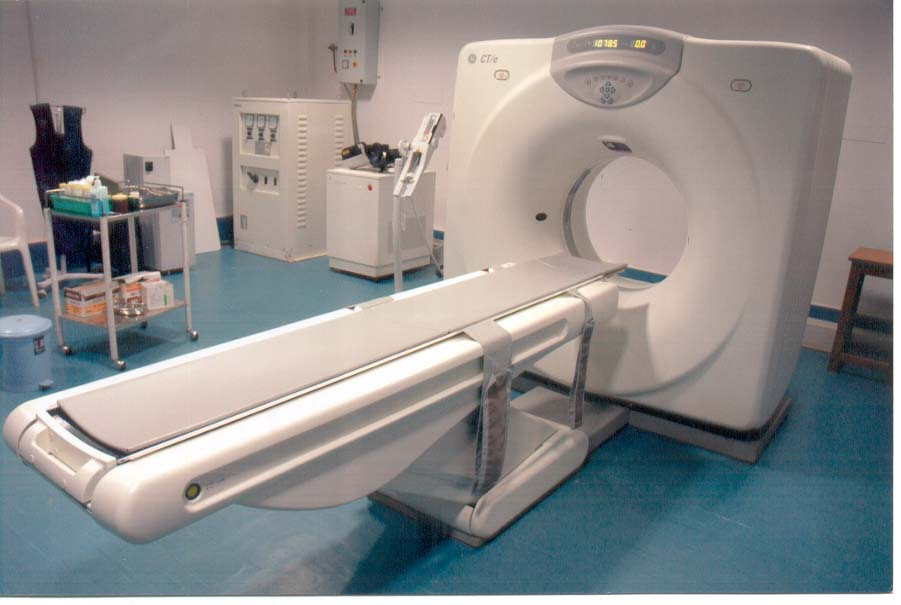
\includegraphics{radon/images/tomograph.jpg}
	\end{adjustbox}
	\caption{Computertomograph \cite{computertomographBild}}
\end{figure}
